A roda omnidirecional aparece em vários modelos na literatura, tais como no design de J. Graboweicki em 1919 \cite{patent_US1305535A} e o de Josef Blumrich em 1972 \cite{patent_US3789947A}. A roda consiste de rolos perpendiculares à  sua direção de giro, cuja presença tem como efeito conferir à roda a capacidade de se locomover em qualquer direção no seu plano. Essa capacidade é o que confere aos robôs aqui discutidos suas características holonômicas, uma vez que as restrições de movimento a que eles estão sujeitos está normalmente atrelada à construção das rodas \cite{TAKAHASHI}.

\begin{figure}[h]
	\centering
	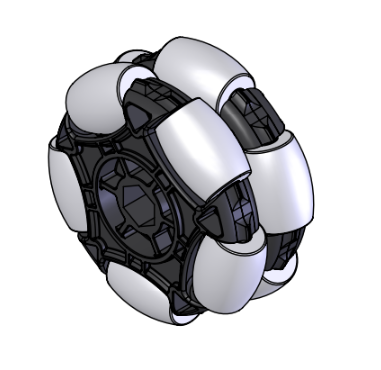
\includegraphics{figures/omniwheel}
	\caption{Modelo de uma Omniwheel \cite{draw_omniwheel}}
\end{figure}

A relação entre velocidade linear e angular da roda é dada por:

\[V_{w1} = \omega_{w1}\cdot r \] 

em que $V_{w}$ é velocidade linear da roda, $r$ o raio da roda, $\omega_{w} $ e é a velocidade angular da roda.

Uma variação da roda omnidirecional é a roda mecanum, criada por Bengt Ilon \cite{patent_US3876255A} - a diferença entre elas é fundamentalmente a construção dos rolos ligados à estrutura central (que, no caso da roda mecanum, são posicionados a 45°).

